\documentclass[a4paper]{beamer}
\usetheme{default}

\usepackage{times}
\usepackage{amsmath}
\usepackage[spanish]{babel}
\usepackage{graphicx}
\usepackage{tikz}
\usepackage{soul}

\title{\vspace{-0.8cm}EL INTERFERÓMETRO}
\author{\vspace{0.2cm}\textit{por Marcos Raúl Gatica}}
\date{}
\begin{document}
	\begin{frame}[plain]
    	\maketitle
    	\vspace{-2cm}
    	\begin{figure}[h!]
    		\centering
    		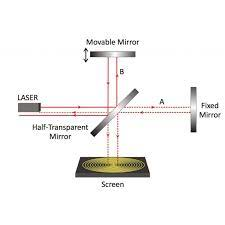
\includegraphics[width=6cm]{../imagenes/interferometro2.jpg}
    	\end{figure}
	\end{frame}
	
	\begin{frame}
   		 \frametitle{\textit{CONCEPTOS PREVIOS}}
   		 
	\end{frame}
	\begin{frame}
		\frametitle{\textit{CONCEPTOS PREVIOS}}
		
		\begin{tikzpicture}[remember picture, overlay]
			\draw[line width=1pt] (-0.4cm, 3.3cm) -- (-0.4cm, -4cm);
		\end{tikzpicture}
	\end{frame}
	
	\begin{frame}
		\frametitle{\textit{CONCEPTOS PREVIOS}}
		
		\begin{tikzpicture}[remember picture, overlay]
			\draw[line width=1pt] (-0.4cm, 3.3cm) -- (-0.4cm, -4cm);
			\draw[line width=1pt] (-0.4cm, 3cm) -- (0cm, 3cm);
			\node at (2cm, 3cm) {\textbf{\textit{La interferencia}}};
		\end{tikzpicture}
	\end{frame}
	
	\begin{frame}
	\frametitle{\textit{CONCEPTOS PREVIOS}}
	
	\begin{tikzpicture}[remember picture, overlay]
		\draw[line width=1pt] (-0.4cm, 3.3cm) -- (-0.4cm, -4cm);
		\draw[line width=1pt] (-0.4cm, 3cm) -- (0cm, 3cm);
		\node at (2cm, 3cm) {\textbf{\textit{La interferencia}}};
		\draw[line width=1pt] (0.8cm, 2.7cm) -- (0.8cm, 2.2cm) -- (1.2cm, 2.2cm);
		\node at (4cm, 2.2cm) {\textit{El principio de superposición}};
	\end{tikzpicture}
	\end{frame}
	
\begin{frame}

	\frametitle{\textit{CONCEPTOS PREVIOS}}
	
	\begin{tikzpicture}[remember picture, overlay]
		\draw[line width=1pt] (-0.4cm, 3.3cm) -- (-0.4cm, -4cm);
		\draw[line width=1pt] (-0.4cm, 3cm) -- (0cm, 3cm);
		\node at (2cm, 3cm) {\textbf{\textit{La interferencia}}};
		\draw[line width=1pt] (0.8cm, 2.7cm) -- (0.8cm, 2.2cm) -- (1.2cm, 2.2cm);
		\node at (4cm, 2.2cm) {\textit{El principio de superposición}};
		\node at (9.5cm, 0cm) {\begin{minipage} [c] {12cm}
				
					${y_1} = A.sen(kx - \omega t)$ \\
					${y_2} = A.sen(kx - \omega t)$ \\ \
					
					${y_{RT}} = {y_1} + {y_2}$ \\
					${y_{RT}} = 2A.sen(kx - \omega t)$ \\
				
		\end{minipage}};
	\end{tikzpicture}
\end{frame}

	\begin{frame}
	\frametitle{\textit{CONCEPTOS PREVIOS}}
	
	\begin{tikzpicture}[remember picture, overlay]
		\draw[line width=1pt] (-0.4cm, 3.3cm) -- (-0.4cm, -4cm);
		\draw[line width=1pt] (-0.4cm, 3cm) -- (0cm, 3cm);
		\node at (2cm, 3cm) {\textbf{\textit{La interferencia}}};
		\draw[line width=1pt] (0.8cm, 2.7cm) -- (0.8cm, 2.2cm) -- (1.2cm, 2.2cm);
		\node at (4cm, 2.2cm) {\textit{El principio de superposición}};
	\end{tikzpicture}
\end{frame}

	\begin{frame}
	\frametitle{\textit{CONCEPTOS PREVIOS}}
	
	\begin{tikzpicture}[remember picture, overlay]
		\draw[line width=1pt] (-0.4cm, 3.3cm) -- (-0.4cm, -4cm);
		\draw[line width=1pt] (-0.4cm, 3cm) -- (0cm, 3cm);
		\node at (2cm, 3cm) {\textbf{\textit{La interferencia}}};
		\draw[line width=1pt] (0.8cm, 2.7cm) -- (0.8cm, 2.2cm) -- (1.2cm, 2.2cm);
		\node at (4cm, 2.2cm) {\textit{El principio de superposición}};
		\draw[line width=1pt] (-0.4cm, 1.4cm) -- (0cm,1.4cm);
		\node at (3.3cm, 1.4cm) {\textbf{\textit{Int. constructiva y destructiva}}};
	\end{tikzpicture}
\end{frame}

	\begin{frame}
	\frametitle{\textit{CONCEPTOS PREVIOS}}
	
	\begin{tikzpicture}[remember picture, overlay]
		\draw[line width=1pt] (-0.4cm, 3.3cm) -- (-0.4cm, -4cm);
		
		\draw[line width=1pt] (-0.4cm, 3cm) -- (0cm, 3cm);
		
		\node at (2cm, 3cm) {\textbf{\textit{La interferencia}}};
		
		\draw[line width=1pt] (0.8cm, 2.7cm) -- (0.8cm, 2.2cm) -- (1.2cm, 2.2cm);
		
		\node at (4cm, 2.2cm) {\textit{El principio de superposición}};
		
		\draw[line width=1pt] (-0.4cm, 1.4cm) -- (0cm,1.4cm);
		
		\node at (3.3cm, 1.4cm) {\textbf{\textit{Int. constructiva y destructiva}}};
		
		\draw[line width=1pt] (0.8cm, 1.1cm) -- (0.8cm, 0.6cm) -- (1.2cm, 0.6cm);
		
		\node at (3.8cm, 0.6cm) {\textit{Interferencia constructiva}};
		
		\node at (12.5cm, 0.5cm)
		{\begin{minipage} [c] {12cm}
		
	     $\Delta L = m . \lambda$ \\
	    
		\end{minipage}};
	
		\draw[line width=1pt] (0.8 cm, 1.1cm) -- (0.8cm, 0.1cm) -- (1.2cm, 0.1cm);
		
		\node at (3.8cm, 0.1cm) {\textit{Interferencia destructiva}};

		\node at (12.5cm, 0cm)
		{\begin{minipage} [c] {12cm}
				
		$\Delta L = (m . {\frac{1}{2}}) . \lambda$
		\end{minipage}};
	\end{tikzpicture}
\end{frame}
%---------------------------------------------
\begin{frame}
	\frametitle{\textit{EL INTERFERÓMETRO}}
\end{frame}

\begin{frame}
	\frametitle{\textit{EL INTERFERÓMETRO}}
	\begin{tikzpicture}[remember picture, overlay]
		\draw[line width=1pt] (-0.4cm, 3.3cm) -- (-0.4cm, -4cm);
	\end{tikzpicture}
\end{frame}

\begin{frame}
	\frametitle{\textit{EL INTERFERÓMETRO}}
	\begin{tikzpicture}[remember picture, overlay]
		\draw[line width=1pt] (-0.4cm, 3.3cm) -- (-0.4cm, -4cm);
		\draw[line width=1pt] (-0.4cm, 3.3cm) -- (-0.4cm, -4cm);
		
		\draw[line width=1pt] (-0.4cm, 3cm) -- (0cm, 3cm);
		
		\node at (4cm, 3cm) {\textbf{\textit{Medir ondas usando la interferencia.}}};
	\end{tikzpicture}
\end{frame}

\begin{frame}
	\frametitle{\textit{EL INTERFERÓMETRO}}
	\begin{tikzpicture}[remember picture, overlay]
		\draw[line width=1pt] (-0.4cm, 3.3cm) -- (-0.4cm, -4cm);
		\draw[line width=1pt] (-0.4cm, 3.3cm) -- (-0.4cm, -4cm);
		
		\draw[line width=1pt] (-0.4cm, 3cm) -- (0cm, 3cm);
		
		\node at (4cm, 3cm) {\textbf{\textit{"Medir ondas usando la interferencia."}}};
		
		\draw[line width=1pt] (-0.4cm, 2.4cm) -- (0cm,2.4cm);
		\node at (3.3cm, 2.4cm) {\textbf{\textit{Usos: Interferometría estelar}}};
	\end{tikzpicture}
\end{frame}

\begin{frame}
	\frametitle{\textit{EL INTERFERÓMETRO}}
	\begin{tikzpicture}[remember picture, overlay]
		\draw[line width=1pt] (-0.4cm, 3.3cm) -- (-0.4cm, -4cm);
		\draw[line width=1pt] (-0.4cm, 3.3cm) -- (-0.4cm, -4cm);
		
		\draw[line width=1pt] (-0.4cm, 3cm) -- (0cm, 3cm);
		
		\node at (4cm, 3cm) {\textbf{\textit{"Medir ondas usando la interferencia."}}};
		
		\draw[line width=1pt] (-0.4cm, 2.4cm) -- (0cm,2.4cm);
		\node at (3.3cm, 2.4cm) {\textbf{\textit{Usos: Interferometría estelar}}};
		
		\node at (5cm, -0.5cm)
		{\begin{minipage} [c] {12cm}
				
		\centering
		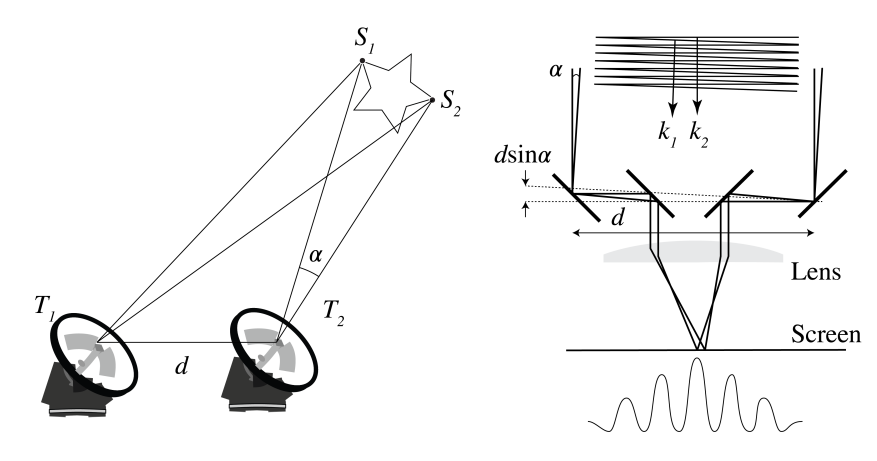
\includegraphics[width = 8cm]{../imagenes/medirEstrellas.jpg}
				
		\end{minipage}};
	\end{tikzpicture}
	
\end{frame}
\begin{frame}
	\frametitle{\textit{EL INTERFERÓMETRO DE MICHELSON}}
	
\end{frame}

\begin{frame}
	\frametitle{\textit{EL INTERFERÓMETRO DE MICHELSON}}
	\begin{tikzpicture}[remember picture, overlay]
		\draw[line width=1pt] (-0.4cm, 3.3cm) -- (-0.4cm, -4cm);
		
	\end{tikzpicture}
\end{frame}
\begin{frame}
	\frametitle{\textit{EL INTERFERÓMETRO DE MICHELSON}}
	\begin{tikzpicture}[remember picture, overlay]
		\draw[line width=1pt] (-0.4cm, 3.3cm) -- (-0.4cm, -4cm);
		\draw[line width=1pt] (-0.4cm, 3.3cm) -- (-0.4cm, -4cm);
		
		\draw[line width=1pt] (-0.4cm, 3cm) -- (0cm, 3cm);
		
		\node at (5cm, 3cm) {\textbf{\textit{Bastante conocido; su estructura básica incluye:}}};
		
	\end{tikzpicture}
\end{frame}
\begin{frame}
	\frametitle{\textit{EL INTERFERÓMETRO DE MICHELSON}}
	\begin{tikzpicture}[remember picture, overlay]
		\draw[line width=1pt] (-0.4cm, 3.3cm) -- (-0.4cm, -4cm);
				\draw[line width=1pt] (-0.4cm, 3.3cm) -- (-0.4cm, -4cm);
		
		\draw[line width=1pt] (-0.4cm, 3cm) -- (0cm, 3cm);
		
		\node at (5cm, 3cm) {\textbf{\textit{Bastante conocido; su estructura básica incluye:}}};
		
		\node at (5cm, 1cm)
		{\begin{minipage} [c] {12cm}
				
		\centering
		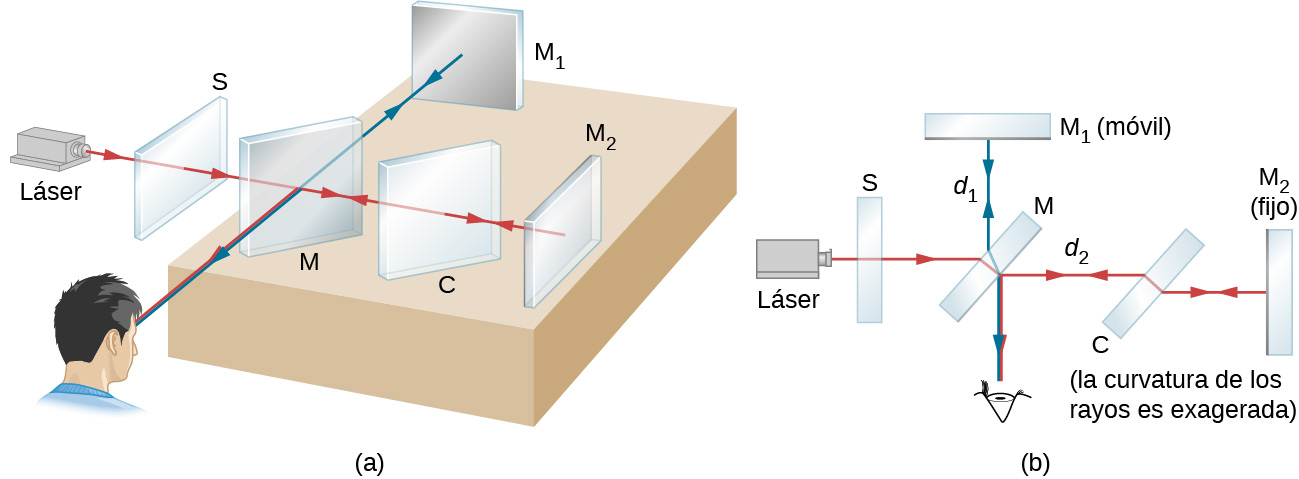
\includegraphics[width = 8cm]{../imagenes/interferometroDibujoCompleto.jpg}
				
		\end{minipage}};
	\end{tikzpicture}
\end{frame}

\begin{frame}
	\frametitle{\textit{EL INTERFERÓMETRO DE MICHELSON}}
	\begin{tikzpicture}[remember picture, overlay]
		\draw[line width=1pt] (-0.4cm, 3.3cm) -- (-0.4cm, -4cm);
		\draw[line width=1pt] (-0.4cm, 3.3cm) -- (-0.4cm, -4cm);
		
		\draw[line width=1pt] (-0.4cm, 3cm) -- (0cm, 3cm);
		
		\node at (5cm, 3cm) {\textbf{\textit{Bastante conocido; su estructura básica incluye:}}};
		
		\node at (5cm, 1cm)
		{\begin{minipage} [c] {12cm}
				
				\centering
				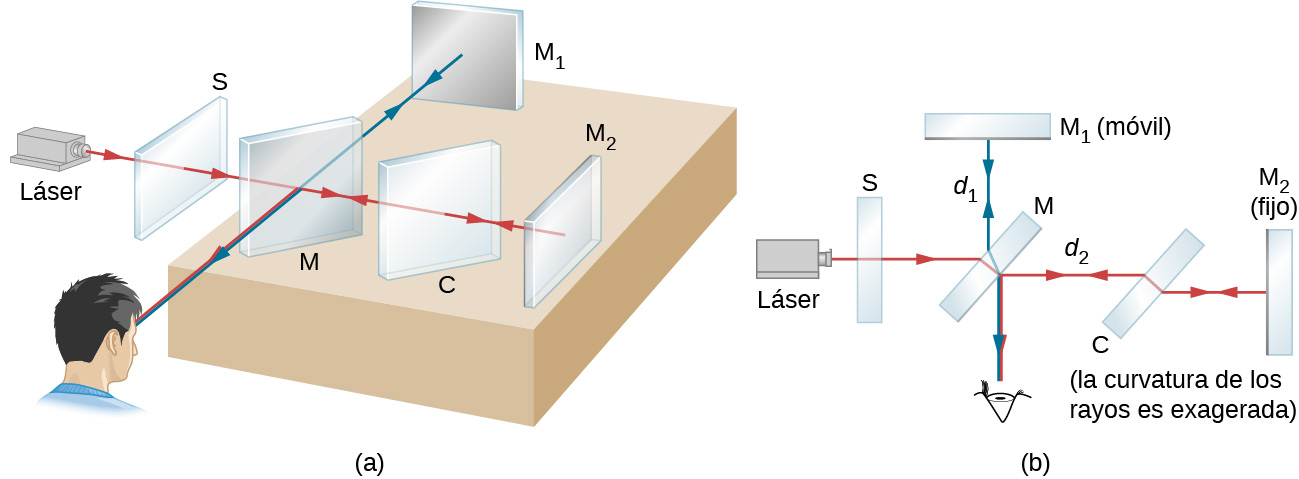
\includegraphics[width = 8cm]{../imagenes/interferometroDibujoCompleto.jpg}
				
		\end{minipage}};
	
		\node at (3cm, -2cm)
		{\begin{minipage} [c] {5cm}
			
			\begin{itemize}
				\item Fuente de luz	
				\item Divisor de haz
			\end{itemize}
		\end{minipage}};
		\node at (8cm, -2.1cm)
		{\begin{minipage} [c] {5cm}
			
			\begin{itemize}
				\item Espejos
				\item Superposición de haces
			\end{itemize}
		\end{minipage}};
	\end{tikzpicture}
\end{frame}

\begin{frame}
	\frametitle{\textit{EL INTERFERÓMETRO DE MICHELSON}}
	\begin{tikzpicture}[remember picture, overlay]
		\draw[line width=1pt] (-0.4cm, 3.3cm) -- (-0.4cm, -4cm);
		\draw[line width=1pt] (-0.4cm, 3.3cm) -- (-0.4cm, -4cm);
		
		\draw[line width=1pt] (-0.4cm, 3cm) -- (0cm, 3cm);
		
		\node at (5cm, 3cm) {\textbf{\textit{Bastante conocido; su estructura básica incluye:}}};
		\node at (5cm, 2.65cm) {\textbf{\textit{...}}};
	\end{tikzpicture}
\end{frame}

\begin{frame}
	\frametitle{\textit{EL INTERFERÓMETRO DE MICHELSON}}
	\begin{tikzpicture}[remember picture, overlay]
		\draw[line width=1pt] (-0.4cm, 3.3cm) -- (-0.4cm, -4cm);
		\draw[line width=1pt] (-0.4cm, 3.3cm) -- (-0.4cm, -4cm);
		
		\draw[line width=1pt] (-0.4cm, 3cm) -- (0cm, 3cm);
		
		\node at (5cm, 3cm) {\textbf{\textit{Bastante conocido; su estructura básica incluye:}}};
		\node at (5cm, 2.65cm) {\textbf{\textit{...}}};
		
		\draw[line width=1pt] (-0.4cm, 2.2cm) -- (0cm,2.2cm);
		\node at (2.6cm, 2.2cm) {\textbf{\textit{Fórmula de Michelson:}}};
	\end{tikzpicture}
\end{frame}

\begin{frame}
	\frametitle{\textit{EL INTERFERÓMETRO DE MICHELSON}}
	\begin{tikzpicture}[remember picture, overlay]
		\draw[line width=1pt] (-0.4cm, 3.3cm) -- (-0.4cm, -4cm);
		\draw[line width=1pt] (-0.4cm, 3.3cm) -- (-0.4cm, -4cm);
		
		\draw[line width=1pt] (-0.4cm, 3cm) -- (0cm, 3cm);
		
		\node at (5cm, 3cm) {\textbf{\textit{Bastante conocido; su estructura básica incluye:}}};
		\node at (5cm, 2.65cm) {\textbf{\textit{...}}};
		
		\draw[line width=1pt] (-0.4cm, 2.2cm) -- (0cm,2.2cm);
		\node at (2.6cm, 2.2cm) {\textbf{\textit{Fórmula de Michelson:}}};
		
		\node at (5cm, 1.4cm)
		{\begin{minipage} [c] {6cm}
			N = $\frac{2 \Delta L}{\lambda}$
		
		\end{minipage}};
	
		\node at (8cm, 0cm)
		{\begin{minipage} [c] {6cm}
			 \begin{itemize}
				\item N: número de franjas de interferencia.
				\item $\Delta L$: diferencia en la longitud de los caminos recorridos por los dos haces de luz.
				\item $\lambda$: longitud de onda de la luz utilizada.
			\end{itemize}
			
		\end{minipage}};
	\end{tikzpicture}
\end{frame}

\begin{frame}
	\frametitle{\textit{EL INTERFERÓMETRO DE MICHELSON}}
	\begin{tikzpicture}[remember picture, overlay]
		\draw[line width=1pt] (-0.4cm, 3.3cm) -- (-0.4cm, -4cm);
		\draw[line width=1pt] (-0.4cm, 3.3cm) -- (-0.4cm, -4cm);
		
		\draw[line width=1pt] (-0.4cm, 3cm) -- (0cm, 3cm);
		
		\node at (5cm, 3cm) {\textbf{\textit{Bastante conocido; su estructura básica incluye:}}};
		\node at (5cm, 2.65cm) {\textbf{\textit{...}}};
		
		\draw[line width=1pt] (-0.4cm, 2.2cm) -- (0cm,2.2cm);
		\node at (2.6cm, 2.2cm) {\textbf{\textit{Fórmula de Michelson:}}};
		
		\node at (8.5cm, 2.15cm)
		{\begin{minipage} [c] {6cm}
				N = $\frac{2 \Delta L}{\lambda}$
				
		\end{minipage}};
	
		\draw[line width=1pt] (-0.4cm, 1.65cm) -- (0cm,1.65cm);
		\node at (2.05cm, 1.65cm) {\textbf{\textit{Funcionamiento:}}};
				
	\end{tikzpicture}
\end{frame}

\begin{frame}
	\frametitle{\textit{EL INTERFERÓMETRO DE MICHELSON}}
	\begin{tikzpicture}[remember picture, overlay]
		\draw[line width=1pt] (-0.4cm, 3.3cm) -- (-0.4cm, -4cm);
		\draw[line width=1pt] (-0.4cm, 3.3cm) -- (-0.4cm, -4cm);
		
		\draw[line width=1pt] (-0.4cm, 3cm) -- (0cm, 3cm);
		
		\node at (5cm, 3cm) {\textbf{\textit{Bastante conocido; su estructura básica incluye:}}};
		\node at (5cm, 2.65cm) {\textbf{\textit{...}}};
		
		\draw[line width=1pt] (-0.4cm, 2.2cm) -- (0cm,2.2cm);
		\node at (2.6cm, 2.2cm) {\textbf{\textit{Fórmula de Michelson:}}};
		
		\node at (8.5cm, 2.15cm)
		{\begin{minipage} [c] {6cm}
				N = $\frac{2 \Delta L}{\lambda}$
				
		\end{minipage}};
		
		\draw[line width=1pt] (-0.4cm, 1.65cm) -- (0cm,1.65cm);
		\node at (2.05cm, 1.65cm) {\textbf{\textit{Funcionamiento:}}};
		
		\node at (5cm, 1cm)
		{\begin{minipage} [c] {9cm}
			Luz coherente (láser) $\rightarrow$ láser/2 (divisor de haces)
				
		\end{minipage}};
		
	\end{tikzpicture}
\end{frame}

\begin{frame}
	\frametitle{\textit{EL INTERFERÓMETRO DE MICHELSON}}
	\begin{tikzpicture}[remember picture, overlay]
		\draw[line width=1pt] (-0.4cm, 3.3cm) -- (-0.4cm, -4cm);
		\draw[line width=1pt] (-0.4cm, 3.3cm) -- (-0.4cm, -4cm);
		
		\draw[line width=1pt] (-0.4cm, 3cm) -- (0cm, 3cm);
		
		\node at (5cm, 3cm) {\textbf{\textit{Bastante conocido; su estructura básica incluye:}}};
		\node at (5cm, 2.65cm) {\textbf{\textit{...}}};
		
		\draw[line width=1pt] (-0.4cm, 2.2cm) -- (0cm,2.2cm);
		\node at (2.6cm, 2.2cm) {\textbf{\textit{Fórmula de Michelson:}}};
		
		\node at (8.5cm, 2.15cm)
		{\begin{minipage} [c] {6cm}
				N = $\frac{2 \Delta L}{\lambda}$
				
		\end{minipage}};
		
		\draw[line width=1pt] (-0.4cm, 1.65cm) -- (0cm,1.65cm);
		\node at (2.05cm, 1.65cm) {\textbf{\textit{Funcionamiento:}}};
		
		\node at (5cm, 1cm)
		{\begin{minipage} [c] {9cm}
				Luz coherente (láser) $\rightarrow$ láser/2 (divisor de haces)
				
		\end{minipage}};
	
		\node at (6.5cm, 0.5cm)
		{\begin{minipage} [c] {12cm}
			Reflexión $\rightarrow$ Interferencia $\rightarrow$ Desplazamientos
		\end{minipage}};
	\end{tikzpicture}
\end{frame}

\begin{frame}
	\frametitle{\textit{EL INTERFERÓMETRO DE MICHELSON}}
	\begin{tikzpicture}[remember picture, overlay]
		\draw[line width=1pt] (-0.4cm, 3.3cm) -- (-0.4cm, -4cm);
		\draw[line width=1pt] (-0.4cm, 3.3cm) -- (-0.4cm, -4cm);
		
		\draw[line width=1pt] (-0.4cm, 3cm) -- (0cm, 3cm);
		
		\node at (5cm, 3cm) {\textbf{\textit{Bastante conocido; su estructura básica incluye:}}};
		\node at (5cm, 2.65cm) {\textbf{\textit{...}}};
		
		\draw[line width=1pt] (-0.4cm, 2.2cm) -- (0cm,2.2cm);
		\node at (2.6cm, 2.2cm) {\textbf{\textit{Fórmula de Michelson:}}};
		
		\node at (8.5cm, 2.15cm)
		{\begin{minipage} [c] {6cm}
				N = $\frac{2 \Delta L}{\lambda}$
				
		\end{minipage}};
		
		\draw[line width=1pt] (-0.4cm, 1.65cm) -- (0cm,1.65cm);
		\node at (2.05cm, 1.65cm) {\textbf{\textit{Funcionamiento:}}};
		

		\node at (5cm, -1.5cm)
		{\begin{minipage} [c] {12cm}
			
			\centering
			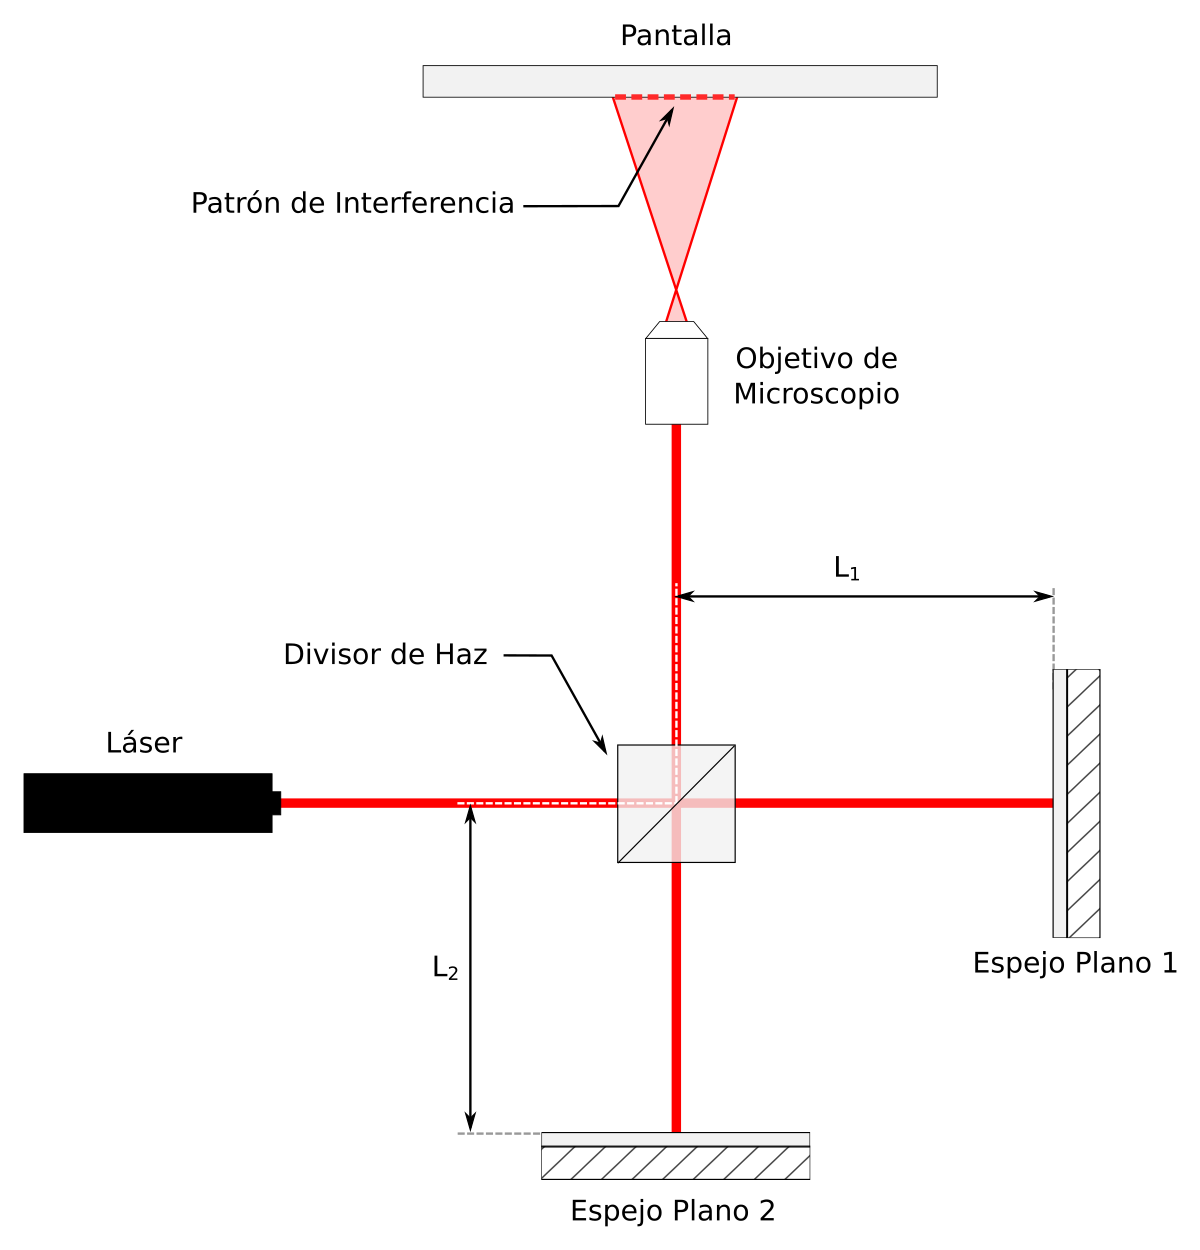
\includegraphics[width = 5cm]{../imagenes/interferometro.png}
			
		\end{minipage}};
	\end{tikzpicture}
\end{frame}

\begin{frame}
	\frametitle{\textit{EXPERIMENTO MICHELSON - MORLEY}}
	
\end{frame}

\begin{frame}
	\frametitle{\textit{EXPERIMENTO MICHELSON - MORLEY}}
	\begin{tikzpicture}[remember picture, overlay]
		\draw[line width=1pt] (-0.4cm, 3.3cm) -- (-0.4cm, -4cm);
		
	\end{tikzpicture}
\end{frame}

\begin{frame}
	\frametitle{\textit{EXPERIMENTO MICHELSON - MORLEY}}
	\begin{tikzpicture}[remember picture, overlay]
		\draw[line width=1pt] (-0.4cm, 3.3cm) -- (-0.4cm, -4cm);
		\draw[line width=1pt] (-0.4cm, 3.3cm) -- (-0.4cm, -4cm);
		
		\draw[line width=1pt] (-0.4cm, 3cm) -- (0cm, 3cm);
		
		\node at (1.5cm, 3cm) {\textbf{\textit{Contexto:}}};
		
	\end{tikzpicture}
\end{frame}
\begin{frame}
	\frametitle{\textit{EXPERIMENTO MICHELSON - MORLEY}}
	\begin{tikzpicture}[remember picture, overlay]
		\draw[line width=1pt] (-0.4cm, 3.3cm) -- (-0.4cm, -4cm);
		\draw[line width=1pt] (-0.4cm, 3.3cm) -- (-0.4cm, -4cm);
		
		\draw[line width=1pt] (-0.4cm, 3cm) -- (0cm, 3cm);
		
		\node at (1.5cm, 3cm) {\textbf{\textit{Contexto:}}};
		\node at (5cm, 0cm)
		{\begin{minipage} [c] {6cm}
				
		\centering
		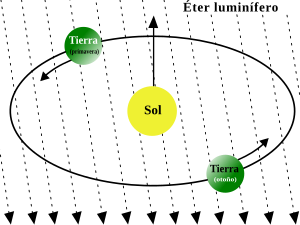
\includegraphics[width = 5cm]{../imagenes/experimentoMM.png}
		\end{minipage}};
	
		\node at (5.5cm, -3cm)
		{\begin{minipage} [c] {8cm}
			\begin{center}
				"Las ondas electromagnéticas como la luz se propagan en el Éter".
			\end{center}
								
		\end{minipage}};
	
	\end{tikzpicture}
\end{frame}
\begin{frame}
	\frametitle{\textit{EXPERIMENTO MICHELSON - MORLEY}}
	\begin{tikzpicture}[remember picture, overlay]
		\draw[line width=1pt] (-0.4cm, 3.3cm) -- (-0.4cm, -4cm);
		\draw[line width=1pt] (-0.4cm, 3.3cm) -- (-0.4cm, -4cm);
		
		\draw[line width=1pt] (-0.4cm, 3cm) -- (0cm, 3cm);
		
		\node at (2.7cm, 3cm) {\textbf{\textit{Contexto: "Luz $\rightarrow$ Éter"}}};
		
	\end{tikzpicture}
\end{frame}
\begin{frame}
	\frametitle{\textit{EXPERIMENTO MICHELSON - MORLEY}}
	\begin{tikzpicture}[remember picture, overlay]
		\draw[line width=1pt] (-0.4cm, 3.3cm) -- (-0.4cm, -4cm);
		\draw[line width=1pt] (-0.4cm, 3.3cm) -- (-0.4cm, -4cm);
		
		\draw[line width=1pt] (-0.4cm, 3cm) -- (0cm, 3cm);
		
		\node at (2.7cm, 3cm) {\textbf{\textit{Contexto: "Luz $\rightarrow$ Éter"}}};
		
		\draw[line width=1pt] (-0.4cm, 2.2cm) -- (0cm,2.2cm);
		\node at (3cm, 2.2cm) {\textbf{\textit{Objetivo y funcionamiento:}}};
				
	\end{tikzpicture}
\end{frame}
\begin{frame}
	\frametitle{\textit{EXPERIMENTO MICHELSON - MORLEY}}
	\begin{tikzpicture}[remember picture, overlay]
		\draw[line width=1pt] (-0.4cm, 3.3cm) -- (-0.4cm, -4cm);
		\draw[line width=1pt] (-0.4cm, 3.3cm) -- (-0.4cm, -4cm);
		
		\draw[line width=1pt] (-0.4cm, 3cm) -- (0cm, 3cm);
		
		\node at (2.7cm, 3cm) {\textbf{\textit{Contexto: "Luz $\rightarrow$ Éter"}}};
		
		\draw[line width=1pt] (-0.4cm, 2.2cm) -- (0cm,2.2cm);
		\node at (3cm, 2.2cm) {\textbf{\textit{Objetivo y funcionamiento:}}};
		
		\node at (5.5cm, 1cm)
		{\begin{minipage} [c] {8cm}
			\begin{center}
					"Determinar la velocidad de la Tierra con respecto al Éter".
			\end{center}
				
		\end{minipage}};
	
	\end{tikzpicture}
\end{frame}
\begin{frame}
	\frametitle{\textit{EXPERIMENTO MICHELSON - MORLEY}}
	\begin{tikzpicture}[remember picture, overlay]
		\draw[line width=1pt] (-0.4cm, 3.3cm) -- (-0.4cm, -4cm);
		\draw[line width=1pt] (-0.4cm, 3.3cm) -- (-0.4cm, -4cm);
		
		\draw[line width=1pt] (-0.4cm, 3cm) -- (0cm, 3cm);
		
		\node at (2.7cm, 3cm) {\textbf{\textit{Contexto: "Luz $\rightarrow$ Éter"}}};
		
		\draw[line width=1pt] (-0.4cm, 2.2cm) -- (0cm,2.2cm);
		\node at (3cm, 2.2cm) {\textbf{\textit{Objetivo y funcionamiento:}}};
		
		\node at (5.5cm, 1cm)
		{\begin{minipage} [c] {8cm}
				\begin{center}
					"Determinar la velocidad de la Tierra con respecto al Éter".
				\end{center}
				
		\end{minipage}};
		\node at (5.5cm, 0cm)
		{\begin{minipage} [c] {8cm}
				\begin{center}
					"La velocidad de la luz debería ser diferente respecto a la orientación del interferómetro".
				\end{center}
				
		\end{minipage}};
	\end{tikzpicture}
\end{frame}
\begin{frame}
	\frametitle{\textit{EXPERIMENTO MICHELSON - MORLEY}}
	\begin{tikzpicture}[remember picture, overlay]
		\draw[line width=1pt] (-0.4cm, 3.3cm) -- (-0.4cm, -4cm);
		\draw[line width=1pt] (-0.4cm, 3.3cm) -- (-0.4cm, -4cm);
		
		\draw[line width=1pt] (-0.4cm, 3cm) -- (0cm, 3cm);
		
		\node at (2.7cm, 3cm) {\textbf{\textit{Contexto: "Luz $\rightarrow$ Éter"}}};
		
		\draw[line width=1pt] (-0.4cm, 2.2cm) -- (0cm,2.2cm);
		\node at (3cm, 2.2cm) {\textbf{\textit{Objetivo y funcionamiento}}};
		
	\end{tikzpicture}
\end{frame}
\begin{frame}
	\frametitle{\textit{EXPERIMENTO MICHELSON - MORLEY}}
	\begin{tikzpicture}[remember picture, overlay]
		\draw[line width=1pt] (-0.4cm, 3.3cm) -- (-0.4cm, -4cm);
		\draw[line width=1pt] (-0.4cm, 3.3cm) -- (-0.4cm, -4cm);
		
		\draw[line width=1pt] (-0.4cm, 3cm) -- (0cm, 3cm);
		
		\node at (2.7cm, 3cm) {\textbf{\textit{Contexto: "Luz $\rightarrow$ Éter"}}};
		
		\draw[line width=1pt] (-0.4cm, 2.2cm) -- (0cm,2.2cm);
		\node at (3cm, 2.2cm) {\textbf{\textit{Objetivo y funcionamiento}}};
		
		\draw[line width=1pt] (-0.4cm, 1.6cm) -- (0cm,1.6cm);
		\node at (1.7cm, 1.6cm) {\textbf{\textit{Resultados:}}};
		
	\end{tikzpicture}
\end{frame}
\begin{frame}
	\frametitle{\textit{EXPERIMENTO MICHELSON - MORLEY}}
	\begin{tikzpicture}[remember picture, overlay]
		\draw[line width=1pt] (-0.4cm, 3.3cm) -- (-0.4cm, -4cm);
		\draw[line width=1pt] (-0.4cm, 3.3cm) -- (-0.4cm, -4cm);
		
		\draw[line width=1pt] (-0.4cm, 3cm) -- (0cm, 3cm);
		
		\node at (2.7cm, 3cm) {\textbf{\textit{Contexto: "Luz $\rightarrow$ Éter"}}};
		
		\draw[line width=1pt] (-0.4cm, 2.2cm) -- (0cm,2.2cm);
		\node at (3cm, 2.2cm) {\textbf{\textit{Objetivo y funcionamiento}}};
		
		\draw[line width=1pt] (-0.4cm, 1.6cm) -- (0cm,1.6cm);
		\node at (1.7cm, 1.6cm) {\textbf{\textit{Resultados:}}};
				\node at (5.5cm, 0.8cm)
		{\begin{minipage} [c] {8cm}
				\begin{center}
					"No hubo desplazamiento apreciable entre las franjas de interferencia".
				\end{center}
		\end{minipage}};

	\end{tikzpicture}
\end{frame}
\begin{frame}
	\frametitle{\textit{EXPERIMENTO MICHELSON - MORLEY}}
	\begin{tikzpicture}[remember picture, overlay]
		\draw[line width=1pt] (-0.4cm, 3.3cm) -- (-0.4cm, -4cm);
		\draw[line width=1pt] (-0.4cm, 3.3cm) -- (-0.4cm, -4cm);
		
		\draw[line width=1pt] (-0.4cm, 3cm) -- (0cm, 3cm);
		
		\node at (2.7cm, 3cm) {\textbf{\textit{Contexto: "Luz $\rightarrow$ Éter"}}};
		
		\draw[line width=1pt] (-0.4cm, 2.2cm) -- (0cm,2.2cm);
		\node at (3cm, 2.2cm) {\textbf{\textit{Objetivo y funcionamiento}}};
		
		\draw[line width=1pt] (-0.4cm, 1.6cm) -- (0cm,1.6cm);
		\node at (1.7cm, 1.6cm) {\textbf{\textit{Resultados:}}};
		\node at (5.5cm, 0.8cm)
		{\begin{minipage} [c] {8cm}
				\begin{center}
					"No hubo desplazamiento apreciable entre las franjas de interferencia".
				\end{center}
		\end{minipage}};
		\node at (5.5cm, -0.3cm)
		{\begin{minipage} [c] {8cm}
				\begin{center}
					"¿Por qué no cambia la velocidad si la Tierra se mueve a través del Éter?".
				\end{center}
		\end{minipage}};
	\end{tikzpicture}
\end{frame}

\begin{frame}
	\frametitle{\textit{EXPERIMENTO MICHELSON - MORLEY}}
	\begin{tikzpicture}[remember picture, overlay]
		\draw[line width=1pt] (-0.4cm, 3.3cm) -- (-0.4cm, -4cm);
		
	\end{tikzpicture}
\end{frame}
\begin{frame}
	\frametitle{\textit{EXPERIMENTO MICHELSON - MORLEY}}
	\begin{tikzpicture}[remember picture, overlay]
		\draw[line width=1pt] (-0.4cm, 3.3cm) -- (-0.4cm, -4cm);
		\draw[line width=1pt] (-0.4cm, 3.3cm) -- (-0.4cm, -4cm);
		
		\draw[line width=1pt] (-0.4cm, 3cm) -- (0cm, 3cm);
		
		\node at (1.3cm, 3cm) {\textbf{\textit{Análisis:}}};

	\end{tikzpicture}
\end{frame}


\begin{frame}
	\frametitle{\textit{EXPERIMENTO MICHELSON - MORLEY}}
	\begin{tikzpicture}[remember picture, overlay]
		\draw[line width=1pt] (-0.4cm, 3.3cm) -- (-0.4cm, -4cm);
		\draw[line width=1pt] (-0.4cm, 3.3cm) -- (-0.4cm, -4cm);
		
		\draw[line width=1pt] (-0.4cm, 3cm) -- (0cm, 3cm);
		
		\node at (1.3cm, 3cm) {\textbf{\textit{Análisis:}}};
		
		\node at (4cm, 1.6cm)
		{\begin{minipage} [c] {8cm}
				"Suponiendo un brazo de interferómetro L, alineado en dirección al movimiento de la Tierra, el tiempo total en ir y volver es:"
		\end{minipage}};
		
		\node at (4cm, 0cm)
		{\begin{minipage} [c] {8cm}
				
${t_{||}} = {\frac{L}{c-v}} + {\frac{L}{c+v}}$ 
		\end{minipage}};
	\end{tikzpicture}
\end{frame}
\begin{frame}
	\frametitle{\textit{EXPERIMENTO MICHELSON - MORLEY}}
	\begin{tikzpicture}[remember picture, overlay]
		\draw[line width=1pt] (-0.4cm, 3.3cm) -- (-0.4cm, -4cm);
		\draw[line width=1pt] (-0.4cm, 3.3cm) -- (-0.4cm, -4cm);
		
		\draw[line width=1pt] (-0.4cm, 3cm) -- (0cm, 3cm);
		
		\node at (1.3cm, 3cm) {\textbf{\textit{Análisis:}}};
		\node at (4cm, 2cm)
		{\begin{minipage} [c] {8cm}
				
				${t_{||}} = {\frac{L}{c-v}} + {\frac{L}{c+v}}$ 
				
				${t_{||}} = {\frac{2L}{c}} . \frac {1}{1- (\frac{v}{c})^2}$ 
				

		\end{minipage}};
		
		
	\end{tikzpicture}
\end{frame}
\begin{frame}
	\frametitle{\textit{EXPERIMENTO MICHELSON - MORLEY}}
	\begin{tikzpicture}[remember picture, overlay]
		\draw[line width=1pt] (-0.4cm, 3.3cm) -- (-0.4cm, -4cm);
		\draw[line width=1pt] (-0.4cm, 3.3cm) -- (-0.4cm, -4cm);
		
		\draw[line width=1pt] (-0.4cm, 3cm) -- (0cm, 3cm);
		
		\node at (1.3cm, 3cm) {\textbf{\textit{Análisis:}}};
		\node at (4cm, 1.6cm)
		{\begin{minipage} [c] {8cm}
				
				${t_{||}} = {\frac{L}{c-v}} + {\frac{L}{c+v}}$ 
				
				${t_{||}} = {\frac{2L}{c}} . \frac {1}{1- (\frac{v}{c})^2}$ 
				
				${t_{||}} \approx {\frac{2L}{c}} (1 + \frac{v^2}{c^2})$
		\end{minipage}};
	
	
	\end{tikzpicture}
\end{frame}
\begin{frame}
	\frametitle{\textit{EXPERIMENTO MICHELSON - MORLEY}}
	\begin{tikzpicture}[remember picture, overlay]
		\draw[line width=1pt] (-0.4cm, 3.3cm) -- (-0.4cm, -4cm);
		\draw[line width=1pt] (-0.4cm, 3.3cm) -- (-0.4cm, -4cm);
		
		\draw[line width=1pt] (-0.4cm, 3cm) -- (0cm, 3cm);
		
		\node at (1.3cm, 3cm) {\textbf{\textit{Análisis:}}};
		\node at (4cm, 1.6cm)
		{\begin{minipage} [c] {8cm}
				
				${t_{||}} = {\frac{L}{c-v}} + {\frac{L}{c+v}}$ 
				
				${t_{||}} = {\frac{2L}{c}} . \frac {1}{1- (\frac{v}{c})^2}$ 
				
				${t_{||}} \approx {\frac{2L}{c}} (1 + \frac{v^2}{c^2})$
		\end{minipage}};
		
		\node at (8cm, 1.6cm)
		{\begin{minipage} [c] {8cm}
				
				$t_{\perp} = \frac{2L}{\sqrt{c^2 - v^2}} = {\frac{2L}{c}} \frac{1}{\sqrt{1 - \frac{v^2}{c^2}}}$
		\end{minipage}};
		\node at (10cm, 1.6cm)
		{\begin{minipage} [c] {2.5cm}
		
		\textit{Tiempo de viaje en perpendicular.}
		\end{minipage}};
	\end{tikzpicture}
\end{frame}

\begin{frame}
	\frametitle{\textit{EXPERIMENTO MICHELSON - MORLEY}}
	\begin{tikzpicture}[remember picture, overlay]
		\draw[line width=1pt] (-0.4cm, 3.3cm) -- (-0.4cm, -4cm);
		\draw[line width=1pt] (-0.4cm, 3.3cm) -- (-0.4cm, -4cm);
		
		\draw[line width=1pt] (-0.4cm, 3cm) -- (0cm, 3cm);
		
		\node at (1.3cm, 3cm) {\textbf{\textit{Análisis:}}};
		\node at (4cm, 1.6cm)
		{\begin{minipage} [c] {8cm}
				
				${t_{||}} = {\frac{L}{c-v}} + {\frac{L}{c+v}}$ 
				
				${t_{||}} = {\frac{2L}{c}} . \frac {1}{1- (\frac{v}{c})^2}$ 
				
				${t_{||}} \approx {\frac{2L}{c}} (1 + \frac{v^2}{c^2})$
		\end{minipage}};
		
		\node at (8cm, 1.6cm)
		{\begin{minipage} [c] {8cm}
				
				$t_{\perp} = \frac{2L}{\sqrt{c^2 - v^2}} = {\frac{2L}{c}} \frac{1}{\sqrt{1 - \frac{v^2}{c^2}}}$
				
				 ${t_{\perp}} \approx {\frac{2L}{c}} (1 + \frac{v^2}{2c^2})$
		\end{minipage}};

	\end{tikzpicture}
\end{frame}

\begin{frame}
	\frametitle{\textit{EXPERIMENTO MICHELSON - MORLEY}}
	\begin{tikzpicture}[remember picture, overlay]
		\draw[line width=1pt] (-0.4cm, 3.3cm) -- (-0.4cm, -4cm);
		\draw[line width=1pt] (-0.4cm, 3.3cm) -- (-0.4cm, -4cm);
		
		\draw[line width=1pt] (-0.4cm, 3cm) -- (0cm, 3cm);
		
		\node at (1.3cm, 3cm) {\textbf{\textit{Análisis:}}};
		\node at (4cm, 1.6cm)
		{\begin{minipage} [c] {8cm}
				
				${t_{||}} = {\frac{L}{c-v}} + {\frac{L}{c+v}}$ 
				
				${t_{||}} = {\frac{2L}{c}} . \frac {1}{1- (\frac{v}{c})^2}$ 
				
				${t_{||}} \approx {\frac{2L}{c}} (1 + \frac{v^2}{c^2})$
		\end{minipage}};
		
		\node at (8cm, 1.6cm)
		{\begin{minipage} [c] {8cm}
				
				$t_{\perp} = \frac{2L}{\sqrt{c^2 - v^2}} = {\frac{2L}{c}} \frac{1}{\sqrt{1 - \frac{v^2}{c^2}}}$
				
				${t_{\perp}} \approx {\frac{2L}{c}} (1 + \frac{v^2}{2c^2})$
		\end{minipage}};
				\node at (8cm, 0cm)
		{\begin{minipage} [c] {8cm}
				
        \hl{$\Delta t = {t_{||}} - {t_{\perp}} = {\frac{2L}{c}} {\frac{v^2}{c^2}}$}
		\end{minipage}};
	\end{tikzpicture}
\end{frame}

\begin{frame}
	\frametitle{\textit{EXPERIMENTO MICHELSON - MORLEY}}
	\begin{tikzpicture}[remember picture, overlay]
		\draw[line width=1pt] (-0.4cm, 3.3cm) -- (-0.4cm, -4cm);
		\draw[line width=1pt] (-0.4cm, 3.3cm) -- (-0.4cm, -4cm);
		
		\draw[line width=1pt] (-0.4cm, 3cm) -- (0cm, 3cm);
		
		\node at (1.3cm, 3cm) {\textbf{\textit{Análisis:}}};
		\node at (4cm, 1.6cm)
		{\begin{minipage} [c] {8cm}
				
				${t_{||}} = {\frac{L}{c-v}} + {\frac{L}{c+v}}$ 
				
				${t_{||}} = {\frac{2L}{c}} . \frac {1}{1- (\frac{v}{c})^2}$ 
				
				${t_{||}} \approx {\frac{2L}{c}} (1 + \frac{v^2}{c^2})$
		\end{minipage}};
		
		\node at (8cm, 1.6cm)
		{\begin{minipage} [c] {8cm}
				
				$t_{\perp} = \frac{2L}{\sqrt{c^2 - v^2}} = {\frac{2L}{c}} \frac{1}{\sqrt{1 - \frac{v^2}{c^2}}}$
				
				${t_{\perp}} \approx {\frac{2L}{c}} (1 + \frac{v^2}{2c^2})$
		\end{minipage}};
		\node at (8cm, 0cm)
		{\begin{minipage} [c] {8cm}
				
				\hl{$\Delta t = {t_{||}} - {t_{\perp}} = {\frac{2L}{c}} {\frac{v^2}{c^2}}$}
		\end{minipage}};
			\node at (5.5cm, -2cm)
	{\begin{minipage} [c] {10cm}
			\begin{center}
				Este desfase era lo que Michelson y Morley esperaban ver cuando giraban el interferómetro 90º, ya que al hacerlo, la diferencia en las trayectorias debería cambiar y causar un desplazamiento en las franjas de interferencia.
			\end{center}
	\end{minipage}};
	\end{tikzpicture}
\end{frame}

\end{document}
